\documentclass[conference]{IEEEtran}
\IEEEoverridecommandlockouts
% The preceding line is only needed to identify funding in the first footnote. If that is unneeded, please comment it out.
\usepackage{cite}
\usepackage{amsmath,amssymb,amsfonts}
\usepackage{algorithmic}
\usepackage{graphicx}
\usepackage{textcomp}
\usepackage{xcolor}
\def\BibTeX{{\rm B\kern-.05em{\sc i\kern-.025em b}\kern-.08em
    T\kern-.1667em\lower.7ex\hbox{E}\kern-.125emX}}

\ifCLASSINFOpdf
\else
    \usepackage[dvips]{graphicx}
\fi
\usepackage{url}
\usepackage{listings}
% \usepackage[margin=1in]{geometry}
\usepackage{amsmath,amsthm,amssymb}
\usepackage{amsmath,amsthm,amssymb}
\usepackage[spanish]{babel} %Castellanización
\usepackage[T1]{fontenc} %escribe lo del teclado
\usepackage[utf8]{inputenc} %Reconoce algunos símbolos
\usepackage{lmodern} %optimiza algunas fuentes
\usepackage{blkarray}
\graphicspath{ {images/} }
\usepackage{hyperref} % Uso de links

\newcommand{\N}{\mathbb{N}}
\newcommand{\Z}{\mathbb{Z}}
\usepackage{float}
\newenvironment{theorem}[2][Theorem]{\begin{trivlist}
\item[\hskip \labelsep {\bfseries #1}\hskip \labelsep {\bfseries #2.}]}{\end{trivlist}}
\newenvironment{lemma}[2][Lemma]{\begin{trivlist}
\item[\hskip \labelsep {\bfseries #1}\hskip \labelsep {\bfseries #2.}]}{\end{trivlist}}
\newenvironment{exercise}[2][Exercise]{\begin{trivlist}
\item[\hskip \labelsep {\bfseries #1}\hskip \labelsep {\bfseries #2.}]}{\end{trivlist}}
\newenvironment{problem}[2][Problem]{\begin{trivlist}
\item[\hskip \labelsep {\bfseries #1}\hskip \labelsep {\bfseries #2.}]}{\end{trivlist}}
\newenvironment{question}[2][Question]{\begin{trivlist}
\item[\hskip \labelsep {\bfseries #1}\hskip \labelsep {\bfseries #2.}]}{\end{trivlist}}
\newenvironment{corollary}[2][Corollary]{\begin{trivlist}
\item[\hskip \labelsep {\bfseries #1}\hskip \labelsep {\bfseries #2.}]}{\end{trivlist}}
\newcommand*{\defeq}{\stackrel{\text{def}}{=}}
\newenvironment{solution}{\begin{proof}[Solution]}{\end{proof}}
\hyphenation{op-tical net-works semi-conduc-tor}

\newcommand{\argmax}{\operatornamewithlimits{argmax}}


\usepackage[ruled,vlined]{algorithm2e}


\begin{document}

\title{Tarea 4. Optimización }

\author{\IEEEauthorblockN{Oscar Esaú Peralta Rosales}
\IEEEauthorblockA{\textit{Maestría en Computación} \\
\textit{Centro de Investigación en Matemáticas}}
}

\maketitle

\begin{abstract}
En esta tarea se realiza la implementación tres métodos de optimización

\begin{itemize}
	\item Cubic interpolation
	\item Barzilai-Borwein
	\item Zhang-Hager
\end{itemize}

y se evalua su comportamiento y resultados con dos tipos de funciones a
optimizar; Rosembrock function, con n = 100 y Wood function.

También se utiliza el método de Barzilai-Borwein para optimizar los parámetros
de para la función de máxima verosimilitud de regresión logística para dos clases y se evalua sobre
el conjunto de datos de imágenes de números MNIST.


\end{abstract}

\begin{IEEEkeywords}
Cubic interpolation, Barzilai-Borwein, Zhang-Hager
\end{IEEEkeywords}

\section{Introduction}

El metodo de Cubic interpolation se basa en la suposición de que tenemos un
intervalo $[a,b]$ en dónde podemos obtener el valor de alǵun tamaño de paso
y dos tamaños de pasos anteriores $\alpha_{i-1}$ y $\alpha_{i-2}$ y una función
cúbica que interpola a $f$ en $\phi(\alpha_{i-1})$, $\phi'(\alpha_{i-1})$,
$\phi(\alpha_{i})$ y $\phi'(\alpha_{i})$. Una vez obtenidos estos valores de
$\alpha$ mediante interpolación elegimos como tamaño de paso (en orden) aquel
que cumpla con las condiciones de Armijo, iterando y reduciendo el intervalo
hasta encontrar alguno.\\

El método de Barzilai-Borwein se basa en encontrar un tamaño de paso $\alpha_k$
tal que $\alpha_k g_k$ aproxime a $H^{-1}g_k$ sin tener que calcular el Hessiano
de la función. El método de Zhang-Hager combina el método anterior con una
técnica de búsqueda en linea no monotónica.\\

Esta ocación usando el método de Barzilai-Borwein se realizó una optimización
sobre los parámetros $\beta$ y $\beta_0$ de la función de máxima verosimilud de
regresion logística para obtener un modelo de clasificación binaria, cuya
función a optimizar para un conjunto de observaciones $S = \{(x_i, y_i\}$ con
$x_i \in R ^{784}$ and $y_i \in \{0, 1\}$ está dada por

\begin{equation}
	h(\beta, \beta_0)= \sum_{i=1}^{n} y_i log\pi_i + (1-y_i)log(1-\pi_i)
\end{equation}

\begin{equation}
	pi_i:= pi_i(\beta, \beta_0) = \frac{1}{1 + \exp(-x_i^T \beta - \beta_0)}
\end{equation}

Aquí cada $x_i$ representa un vector con los valores de los pixeles de una
imagen del dataset de $MINIST$ mencionado anteriormente y $y_i$ representa la
etiqueta asociada a dicha imagen.

\section{Métodología}

\subsection{Implementación de los métodos de cubic interpolation, Barzilai-Borwein
y Zhang-Hager}


Para la implementación del método usando interpolación cúbica usamos la condición de Armijo
$f(x_k + \alpha_k d_k) < f(x_k) + c_1 \alpha_k g_k^T d_k$ para verificar que alguna
$\alpha_0, \alpha_1, \alpha_2$ la cumplan, y en donde definimos:
$\phi(\alpha_k) = f(x_k - \alpha_k g_k)$,
$\phi(0) = f(x_k)$,
$\phi'(0) = - g_k^Tg_k$
$\alpha_1 = \frac{- \alpha_0^2 \phi'(0)}{2 (\phi(\alpha) - \phi'(0) \alpha_0 - \phi(0))}$,
$\alpha_2 = \frac{-b + \sqrt{b^2 - 3ac}}{3a}$ con $c = \phi(0)$ y

$$
\begin{pmatrix}
	a\\
	b\\
\end{pmatrix} =
\frac{1}{\alpha_1^2\alpha_0^2(\alpha_1 - \alpha_0)}
\begin{pmatrix}
	\alpha_0^2 & -\alpha_1^2\\
	\alpha_0^3 & \alpha_1^3\\
\end{pmatrix}
\begin{pmatrix}
	\phi(\alpha_1) - \phi'(0)\alpha_1 - \phi(0)\\
	\phi(\alpha_0) - \phi'(0)\alpha_0 - \phi(0)\\
\end{pmatrix}
$$ \\

En el metodo de Barzilai-Borwein la actualización del tamaño de paso se realiza en cada iteración de
la forma $s_{k-1} = x_k - x_{k-1}$, $y_{k+1} = g_k - g_{k-1}$,
$\alpha_k = \frac{s_{k-1}^T  y_{k+1}}{y_{k+1}^T y_{k+1}}$. \\

Para la implementación del algoritmo de Zhang-Hager se optó por retomar el algoritmo que usa
interpolación cúbica y agregarle la modificación a la condición de Armijo mediante el parámetro
$c_k$, por tanto la condición de Armijo ahora es
$f(x_k + \alpha_k d_k) < c_k + c_1 \alpha_k g_k^T d_k$ donde en cada paso se actualiza con
$q_{k-1} = q_k$, $q_k = \eta  q_k + 1$, $c_k = (\eta  q_{k-1}  c_k + f(x_k)) / q_k$. \\

Puesto que se requiere para algunos cálculos el $\alpha$ anterior para los tres algoritmos se
propuso un $\alpha$ inicial en el rango de $1e^{-3}$.

Para la función de Rosembrock con n=100 se usó un $x$ inicial igual a
$x = [-1.2, 1, 1, ..., 1, -1.2, 1]^T$ cuyo valor óptimo es $x = [1,1,...,1,1]^T$.

Para la función de Wood se usó un $x$ inicial igual a
$x = [-3, -1, -3, -1]^T$ cuyo valor óptimo es $x = [1, 1, 1, 1]^T$.

En la siguiente sección se muestran los resultados obtenidos.

También se muestran los algoritmos implementados en el Apéndice V-B.

\subsection{Optimización sobre modelo de regresión logística binario}

Dado que la el modelo representado por $(1)$ y $(2)$ es para clasificación
binaria se seleccionó solo los imágenes correspondientes a las etiquetas 0 y 1
y con ellas se procedió a optimizar los valores de $\beta$ y $\beta_0$

Para una mejor implementación se procedió a reescribir las ecuaciones (1) y (2)
de la siguiente forma.

Sea $\phi = [\beta, \beta_0]$ y $W = \{w_i\}$ donde $w_i = [x_i, 1]$, con ello
podemos reescribir (1) y (2) como:

\begin{equation}
	h(\phi) = \sum_{i=1}^{n} y_i log\pi_i + (1-y_i)log(1-\pi_i)
\end{equation}

\begin{equation}
	\pi_i:= \pi_i(\phi) = \frac{1}{1 + \exp(-w_i^T\phi)}
\end{equation}

Así el gradiente de $h$ esta dado por:

\begin{equation}
	\nabla_\phi \pi_i(\phi) = \pi_i(\phi)(1 - \pi_i(\phi)) w_i
\end{equation}


\begin{equation*}
	\nabla_\phi h(\phi) = \sum_{i=1}^{n} y_i \frac{\nabla_\phi \pi_i(\phi)}{\pi_i(\phi)} + (1-y_i) \frac{\nabla_\phi (1- \pi_i(\phi))}{1 - \pi_i(\phi)}
\end{equation*}

\begin{equation}
	\nabla_\phi h(\phi) = \sum_{i=1}^{n} y_i (1 - \pi_i(\phi)) - (1-y_i) \pi_i(\phi)
\end{equation}

Para la optimización de sobre los parámetros $\beta$ y $\beta_0$ se decició usar el algoritmo de
Barzilai-Borwein.

El conjunto de datos está dividido en 3 partes, el conjunto de entrenamiento, el conjunto de
validación y el conjunto de prueba.

La optimización de la función se realizó usando el conjunto de entrenamiento, y para su verificación
se procedió a calcular el error obtenido al clasificar el conjunto de validación mediante la
siguiente fórmula:

$$
error = \frac{1}{|\tau|} \sum_{x_i,y_i \in \tau} |1_{\pi_{i}(\phi)}(w_i) - y_i|
$$


En la siguiente sección se muestran los resultados obtenidos.

\section{Resultados}

De las diversas ejecuciones, en las tablas I y II se muestran los mejores resultados obtenidos,
para la aproximación del optimo para la función de Rosembrock y Wood respectivamente.

\begin{table}[htbp]
    \caption{Tabla comparativa entre los 3 métodos con la función de Rosembrock}
    \begin{center}
        \begin{tabular}{|c|c|c|c|}
            \hline
			\textbf{\textit{Algoritmo}}& \textbf{\textit{Iteraciones}}& \textbf{\textit{$||g_k||$}}& \textbf{\textit{$|f(x_k) - f(x^*)|$}} \\

            \hline
            Cubic Interpolation& 10000 & 9.9977 & 3.9866 \\
            Barzilai-Borwein& 953 & 10.0000 & 1.5070e-10 \\
            Zhang-Hager& 10000 & 9.9977 & 3.9866 \\
            \hline
            \multicolumn{4}{l}{}
        \end{tabular}
        \label{tab1}
    \end{center}
\end{table}

\begin{table}[htbp]
    \caption{Tabla comparativa entre los 3 métodos con la función de Wood}
    \begin{center}
        \begin{tabular}{|c|c|c|c|}
            \hline
			\textbf{\textit{Algoritmo}}& \textbf{\textit{Iteraciones}}& \textbf{\textit{$||g_k||$}}& \textbf{\textit{$|f(x_k) - f(x^*)|$}} \\

            \hline
            Cubic Interpolation& 10000 & 1.9180 & 7.8769 \\
            Barzilai-Borwein& 207 & 2.0000 & 3.2988e-15 \\
            Zhang-Hager& 10000 & 1.9180 & 7.8769 \\
            \hline
            \multicolumn{4}{l}{}
        \end{tabular}
        \label{tab2}
    \end{center}
\end{table}

Usando el método de Barzilai-Borwein para la clasificación de las imágenes se obtuvo un error de
0.00047, es decir clasificó correctamente las imagenes con probabilidad de mas 0.9995 de acertar.

La figura \ref{f2} se muestra la imagen formada por la optimización de las $\phi$ la cual representa
algo paracido a un enmascaramiento de las carácterísticas distintivas de las imagenes conformadas de
ceros y unos y que ayuda a clasificarlas correctamente.

% \begin{figure}[htbp]
%     \centerline{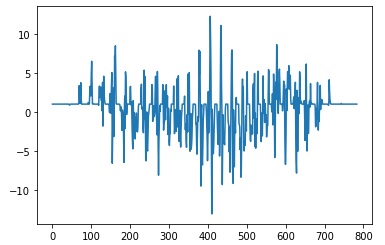
\includegraphics[scale=0.6]{1.png}}
%     \caption{Obtención del minimizador para la función con $\lambda=1$, se observa una buena aproximación sobre los la serie formada por el vector Y.}
%     \label{f1}
% \end{figure}

\begin{figure}[htbp]
    \centerline{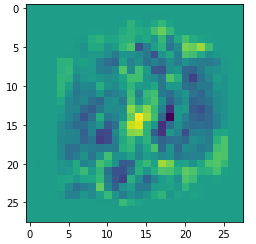
\includegraphics[scale=0.6]{2.png}}
    \caption{Máscara generada por los valores optimizados de $\beta$ usada para clasificar las imágenes de números de 0's y 1's.}
    \label{f2}
\end{figure}

\section{Conclusiones}

Como se ve en los resultados el método de Barzilai-Borwein fue con el que mejores aproximaciones se
obtuvieron, la elección de un $\alpha = 1e-2$ fue crucial para obtener un biuen resultado con la
función de Rosembrock puesto al parecer este tamaño de paso inicial hace que salga de un mínimo
local.\\

La clasificación de las imágenes usando el método de Barzilai-Borwein fue bastante bueno puesto que
se clasificó un conjunto de datos completamente nuevo con un error aproximado de 0.00047. La imagen
mostrada de la representación grafica de los $\beta$ optimizado parece capturar información tal que
le ayuda a decirdir a que clase pertenece, intuitivamente parace que el centro lo usa para identicar
si es o no es un cero, por la forma que esta presenta.

\section{Apéndice}

\subsection{Problemas}

\subsubsection*{1}

Sea $f: \mathcal{R} \rightarrow \mathcal{R}$ dado por $f(x) = (x-a)^4$, donde $a$ es una constante.
Supon que aplicamos el Método de Newton al problema de minimizar $f$.

\begin{itemize}
	\item a) Desarrolla la ecuación de actualización para el Método de Newton aplicado al problema.
	\item b) Sea $y_{k} = | x_{k} - a|$ donde $x_{k}$ es la k-ésima iteración del Método de\
	Newton. Muestra que la secuencia $\{y_{k}\}$  satisface que $y_{k+1} = \frac{2}{3}y_{k}$.
	\item c) Muestra que $x_{k} \rightarrow a$ para cualquier valor inicial $x_{0}$.
	\item d) ¿Cuál es el orden de convergencia de la secuencia $\{x_{k}\}$?.
	\item e) ¿El orden de convergencia anterior contradice el teorema a cerca de la convergencia del\
	del Método de Newton?
\end{itemize}


\textbf{Solución}


\subsubsection*{a}

Sabemos que la dirección de descenso para una serie $\{x_k\}$ generada por el Método de Newton está
dado por $d_k = -H(x_k)^{-1}g(x_k) = x_{k+1} - x_k$ por lo tanto
$x_{k+1} = x_k - -H(x_k)^{-1}g(x_k)$. Para este caso $x_{k+1} = x_k - \frac{f'(x_k)}{f''(x_k)}$,
donde $f'(x) = 4(x-a)^3$ y $f''(x) = 12(x-a)^2$.

Sustituyendo en la fórmula de actualización tenemos que
$x_{k+1} = x_k - \frac{4(x_k-a)^3}{12(x_k-a)^2}$ y finalmente $x_{k+1} = x_k - \frac{1}{3}(x_k-a)$\\

\subsubsection*{b}

Del punto anterior tenemos que $x_{k+1} = x_k - \frac{1}{3}(x_k-a)$, como $y_{k} = | x_{k} - a|$
entonces $y_{k+1} = |x_{k+1} - a|$, sustituyendo $x_{k+1}$ tenemos que
$y_{k+1} = |x_k - \frac{1}{3}(x_k-a) - a| = |x_k - \frac{1}{3}x_k + \frac{1}{3}a - a|$
y finalmente $y_{k+1} = \frac{2}{3} |x_k -a| = \frac{2}{3}y_k$\\

\subsubsection*{c}

Queremos mostrar que $\lim_{k \to \infty}x_k = a$ valor inicial $x_{0}$,
reescribiendo $\lim_{k \to \infty}x_k - a=0$
o también podemos verlo como $\lim_{k \to \infty}y_k=0$ si tomamos la siguiente iteración también
debe cumplirse que $\lim_{k \to \infty}y_{k+1}=0$ o que $\lim_{k \to \infty}\frac{2}{3}y_{k}=0$.

Observemos que $y_1 = \frac{2}{3}y_0$, $y_2 = (\frac{2}{3})^2y_0$, ... $y_k = (\frac{2}{3})^ky_0$.
Luego $\lim_{k \to \infty}(\frac{2}{3})^ky_{0}=0$ puesto que $\frac{2}{3})^k$ tiene a ser cada vez
más pequeño. Así $x_{k} \rightarrow a$ para cualquier valor inicial $x_{0}$.\\

\subsubsection*{d}

Por definición, una sucesión $\{x_k\}$ converge a $L$ con orden $q$ si
$\lim_{k \to \infty} \frac{|x_{k+1} - L|}{|x_k - L|^q} = \mu$ para $\mu > 0$. Ya demostramos que
$x_{k} \rightarrow a$ y tomemos $q=1$ por primero demostrar que tiene convergencia lineal,
entonces, $\lim_{k \to \infty} \frac{|x_{k+1} - a|}{|x_k - a|} = \mu$, sustituyendo tenemos que
$$
\lim_{k \to \infty} \frac{|x_{k+1} - a|}{|x_k - a|} = \lim_{k \to \infty} \frac{y_{k+1}}{y_k}
$$
$$
\lim_{k \to \infty} \frac{|x_{k+1} - a|}{|x_k - a|} = \lim_{k \to \infty} \frac{2y_{k}}{3y_k}
$$
$$
\lim_{k \to \infty} \frac{|x_{k+1} - a|}{|x_k - a|} = \frac{2}{3}
$$

así tenemos que $\mu = \frac{2}{3} > 0$ y por tanto la serie $x_k$ tiene orden de
convergencia lineal.\\


\subsubsection*{e}

La definición de convergencia al menos cuadrática del Método Newton es asegurada para cualquier
punto suficientemente cerca a la solución y que $H(x*)$ sea invertible sin embargo notemos que
la convergencia a $a$ ha sido comprobada para cualquier punto unicial y $f''(a) = 12(a - a)^2 = 0$
por tanto no se cumple con los criterios mencionados anteriormente y no contradice la definición.

\subsection{Algoritmos}

\begin{algorithm}[]
    \SetAlgoLined
    \KwResult{$x_k$}
	$x_k$ <- Inicializar \\
	$g_k$ <- $\nabla f(x)$ \\
	$tol$ <- Inicializar Tolerancia \\
	$\alpha_k$ <- Inicializar alpha inicial \\
	$\alpha_0$ <- $\alpha_k$ \\
	$\alpha_1$, $\alpha_2$ \\
    \While{$||g_k|| > tol$}{
		$\alpha_0 = \alpha_k$ \\
		\If{!armijo($x_k$, $g_k$, $alpha_0$)}{
			$\alpha_1$ = computeAlpha1($x_k$, $g_k$, $\alpha_0$)\\
			\If{armijo($x_k$, $g_k$, $\alpha_1$)}{
				$\alpha_k$ = $\alpha_1$ \\
			}
            \Else {
                $\alpha_2$ = computeAlpha2($x_k$, $g_k$, $\alpha_0$, $\alpha_1$)\\
				\While{!armijo($x_k$, $g_k$, $\alpha_2$)}{
					$\alpha_0$ = $\alpha_1$\\
                    $\alpha_1$ = $\alpha_2$\\
                    $\alpha_2$ = computeAlpha2($x_k$, $g_k$, $\alpha_0$, $\alpha_1$) \\
				}
                $\alpha_k$ = $\alpha_2$ \\
			}
		}
		$x_k$ = $x_k$ - $\alpha_k g_k$\\
		$g_k = g(x_k)$\\
	 }
     \caption{Linear Search with Cubic Interpolation}
\end{algorithm}

\begin{algorithm}[]
    \SetAlgoLined
    \KwResult{$x_k$}
	$x_k$ <- Inicializar \\
	$x_{k-1}$ <- NULL \\
	$g_k$ <- $\nabla f(x)$ \\
	$g_{k-1}$ <- NULL \\
	$tol$ <- Inicializar Tolerancia \\
	$\alpha_k$ <- Inicializar alpha inicial \\
	$k=0$
    \While{$||g_k|| > tol$}{
		\If{$k!=0$}{
			$s_{k-1} = x_k - x_{k-1}$\\
            $y_{k+1} = g_k - g_{k-1}$\\
            $\alpha_k = \frac{s_{k-1}^T  y_{k+1}}{y_{k+1}^T y_{k+1}}$\\
		}
		$x_{k-1} = x_k$\\
		$x_k$ = $x_k$ - $\alpha_k g_k$\\
		$g_{k-1} = g_k$\\
		$g_k = g(x_k)$\\
	 }
     \caption{Barzilai-Borwein}
\end{algorithm}


\begin{algorithm}[]
    \SetAlgoLined
    \KwResult{$x_k$}
	$x_k$ <- Inicializar \\
	$g_k$ <- $\nabla f(x)$ \\
	$c_k$ <- $f(x)$ \\
	$q_k$ <- Inicializar \\
	$q_{k-1}$ <- NULL \\
	$\eta$ <- $f(x)$ \\
	$tol$ <- Inicializar Tolerancia \\
	$\alpha_k$ <- Inicializar alpha inicial \\
	$\alpha_0$ <- $\alpha_k$ \\
	$\alpha_1$, $\alpha_2$ \\
    \While{$||g_k|| > tol$}{
		$\alpha_0 = \alpha_k$ \\
		\If{!armijo($x_k$, $g_k$, $alpha_0$, $c_k$)}{
			$\alpha_1$ = computeAlpha1($x_k$, $g_k$, $\alpha_0$)\\
			\If{armijo($x_k$, $g_k$, $\alpha_1$, $c_k$)}{
				$\alpha_k$ = $\alpha_1$ \\
			}
            \Else {
                $\alpha_2$ = computeAlpha2($x_k$, $g_k$, $\alpha_0$, $\alpha_1$)\\
				\While{!armijo($x_k$, $g_k$, $\alpha_2$, $c_k$)}{
					$\alpha_0$ = $\alpha_1$\\
                    $\alpha_1$ = $\alpha_2$\\
                    $\alpha_2$ = computeAlpha2($x_k$, $g_k$, $\alpha_0$, $\alpha_1$) \\
				}
                $\alpha_k$ = $\alpha_2$ \\
			}
		}
		$x_k$ = $x_k$ - $\alpha_k g_k$\\
		$g_k = g(x_k)$\\

		$q_{k-1} = q_k$\\
        $q_k = \eta  q_k + 1$\\
        $c_k = (\eta  q_{k-1}  c_k + f(x_k)) / q_k$\\
	 }
     \caption{Zhang-Hager}
\end{algorithm}

\section*{}

\begin{thebibliography}{00}
\bibitem{b1} Jorge Nocedal, Stephen J. Wright, ``Numerical Optimization,'' Second Edition, Springer.
\end{thebibliography}

\end{document}
